
\section{定义与基本性质}

\textbf{21.2.1. 仿射情形：三个定义。}\quad 我们首先研究仿射情形。设 $A$ 是一个 $B$-代数，于是我们有\trRing{}的一个\trMorphism{} $\phi\colon B\to A$ 与\trScheme{}的一个\trMorphism{} $\Spec A\to\Spec B$。我将用三种方式定义一个 $A$-模 $\Omega_{A/B}$。它称作\textbf{相对\trDifferential{}模}（module of relative differentials）或\textbf{\trKahlerDifferentials{}模}（module of Kähler differentials）。\trDifferential{}模将定义为这个模，连同一条满足下列三条性质的映射 $\mathrm{d}\colon A\to\Omega_{A/B}$。（当心：尽管 $\mathrm{d}$ 把一个 $A$-模送到一个 $A$-模，它一般却不是 $A$-线性的。先验地我们把它当作\trAbelianGroups{}的一个\trHomomorphism，但稍后马上就会让它成为 $B$-模的\trHomomorphism，见\mbox{练习~21.2.A}。）

（i）\emph{可加性}（additivity）：$\mathrm{d}a+\mathrm{d}a'=\mathrm{d}(a+a')$。

（ii）\emph{\trLeibniz}：$\mathrm{d}(aa')=a\,\mathrm{d}a'+a'\,\mathrm{d}a$。

（iii）\emph{在\trPullback{}上的平凡性}（triviality on pullbacks）：对 $b\in\phi(B)$，$\mathrm{d}b=0$。

若你在任何别的语境里见过\trDifferential，这些性质都不会令人惊讶。

\textbf{21.2.A.（平凡练习）}\quad 证明：$\mathrm{d}$ 是 $B$-线性的。

\textbf{21.2.B.（练习）}\quad 证明商法则（quotient rule）：若 $a'=as$，则 $s^2\,\mathrm{d}a=s\,\mathrm{d}a'-a'\,\mathrm{d}s$。

\textbf{21.2.C.（练习）}\quad 叙述并证明 $\mathrm{d}(f(g))$ 的链式法则（chain rule），其中 $f$ 是带 $B$-系数的一个多项式，而 $g\in A$。（作为动机，想一想 $B=k$ 的情形。于是比如 $\mathrm{d}a^n=na^{n-1}\,\mathrm{d}a$，而更一般地，若 $f$ 是一个变元的多项式，则 $\mathrm{d}f(a)=f'(a)\,\mathrm{d}a$，其中 $f'$ 是形式地定义的：若 $f=\sum c_ix^i$，则 $f'=\sum c_iix^{i-1}$。）

现在我们将看到\trKahlerDifferentials{}模的三个定义，它们不久之后就会「层化」为相对\trDifferential{}的层。第一个定义是具体的、可动手操作的。第二个以\trUniversalProperty{}给出。第三个则整体化良好，将使我们在一般情形下也能方便地定义 $\Omega_{X/Y}$。

\textbf{21.2.2. \trDifferential{}的第一个定义：显式描述。}\quad 我们把 $\Omega_{A/B}$ 定义为符号「$\mathrm{d}a$」（$a\in A$）的有限 $A$-线性组合，但须服从上述三条规则（i）--（iii）。例如取 $A=k[x,y]$、$B=k$，那么一个样品\trDifferential{}是 $3x^2\,\mathrm{d}y+4\,\mathrm{d}x\in\Omega_{A/B}$。我们有诸如下列的恒等式：$\mathrm{d}(3xy^2)=3y^2\,\mathrm{d}x+6xy\,\mathrm{d}y$。

\textbf{21.2.3. 关键事实。}\quad 注意，若 $A$ 在 $B$ 上（作为代数）由一些 $x_i\in A$ 生成（其中 $i$ 属于某个指标集，可以无穷），并服从某些关系 $r_j$（其中 $j$ 属于某个指标集，且每条关系都是诸 $x_i$ 的一个多项式），则 $A$-模 $\Omega_{A/B}$ 由诸 $\mathrm{d}x_i$ 生成，且服从关系 $\mathrm{d}r_j=0$。简言之，我们不必取遍 $A$ 的每一个元素，而可以取一个生成集；我们也不必取这些生成元之间的每一条关系，而可以取诸关系的一些生成元。

\textbf{21.2.D.（练习）}\quad 验证\mbox{关键事实~21.2.3}。（如果你愿意，可以用仿射\trConormal{}正合列，即\mbox{定理~21.2.12}，来验证它；不同的人喜欢以不同的顺序梳理这套理论。只须当心不要陷入循环论证。）

特别地：

\textbf{21.2.4.\ \trhProposition。}\ ——\ \emph{若 $A$ 是\trFinitelyGenerated{} $B$-代数，则 $\Omega_{A/B}$ 是一个有限型（即\trFinitelyGenerated{}）的 $A$-模。若 $A$ 是\trFinitelyPresented{} $B$-代数，则 $\Omega_{A/B}$ 是一个\trFinitelyPresented{} $A$-模。}

回忆（\S8.3.13）：称一个环 $A$ 在另一个环 $B$ 上是\emph{\trFinitelyPresented}的，若它能以有限多个生成元与有限多条关系表出：
\[
A=B[x_1,\dots,x_n]/(r_1(x_1,\dots,x_n),\dots,r_j(x_1,\dots,x_n)).
\]
若 $A$ 是\trNoetherian{}的，则「\trFinitelyPresented」与「有限型」是一回事，因为「有限多条关系」是白送的，所以你们大多数人不必在意。

现在我们来看几个例子。这些例子中有三个是环映射特别重要的构件：添加自由变元、取\trLocalization、取商。如果我们知道如何处理这三件事，我们就知道（至少在理论上）如何处理任何环映射。（在 \S10.2 中实际理解\trFiberProduct{}时，它们也曾同样有用。）

\textbf{21.2.5. 例子：取商。}\quad 若 $A=B/I$，则 $\Omega_{A/B}=0$：对一切 $a\in A$，$\mathrm{d}a=0$，因为每个这样的 $a$ 都是 $B$ 中某个元素的像。这应当是可信的；此时不存在「相对\trTangentVector」。

\textbf{21.2.6. 例子：添加变元。}\quad 若 $A=B[x_1,\dots,x_n]$，则 $\Omega_{A/B}=A\,\mathrm{d}x_1\oplus\cdots\oplus A\,\mathrm{d}x_n$。（注意，即使我们添加任意无穷多个未定元，这一论证也适用。）这背后的直观几何使得答案非常合理。仿射 $n$-空间的\trCotangentBundle{}确实应当是秩 $n$ 的自由模。

\textbf{21.2.7. 显式例子：一条仿射平面曲线。}\quad 考虑 $\mathbb{A}^2_k$ 中的平面曲线 $y^2=x^3-x$，其中 $k$ 的\trCharacteristic{}不是 $2$（其图像见图~19.7）。令 $A=k[x,y]/(y^2-x^3+x)$、$B=k$。由\mbox{关键事实~21.2.3}，\trDifferential{}模 $\Omega_{A/B}$ 由 $\mathrm{d}x$ 与 $\mathrm{d}y$ 生成，且服从关系
\[
2y\,\mathrm{d}y=(3x^2-1)\,\mathrm{d}x.
\]
于是在 $y\ne 0$ 的轨迹上，$\mathrm{d}x$ 是一个生成元（因为 $\mathrm{d}y$ 可以用 $\mathrm{d}x$ 表出）。我们得出：在 $y\ne 0$ 的轨迹上，$\widetilde{\Omega}_{A/B}$ 同构于平凡\trLineBundle{}（即\trInvertibleSheaf）。类似地，在 $3x^2-1\ne 0$ 的轨迹上，$\mathrm{d}y$ 是一个生成元。这两块轨迹盖满了整条曲线，因为解 $y=0$ 给出 $x^3-x=0$，即 $x=0$ 或 $\pm 1$，而在这些情形的每一处都有 $3x^2-1\ne 0$。我们已经证明了 $\widetilde{\Omega}_{A/B}$ 是一个\trInvertibleSheaf。

我们可以几何地诠释 $\mathrm{d}x$ 与 $\mathrm{d}y$。\trDifferential{} $\mathrm{d}x$ 在哪里消失？上一段表明它在 $2y\ne 0$ 的块上不消失。在 $3x^2-1\ne 0$ 的块上（$\mathrm{d}y$ 在此是生成元），$\mathrm{d}x=(2y/(3x^2-1))\,\mathrm{d}y$，由此可见 $\mathrm{d}x$ 恰在 $y=0$ 处消失。看着图像，你应当觉得可信。我们已经证明了：$\mathrm{d}x=0$ 恰在这条曲线具有竖直\trTangentVector{}的地方成立。一旦我们能够拉回\trDifferential（\mbox{练习~21.2.K(a)} 或\mbox{定理~21.2.26}），我们就可以把 $\mathrm{d}x$ 诠释为 $x$-轴上一个\trDifferential{}拉回到 $\Spec A$ 的结果（沿向 $x$-轴的\trProjection{}作拉回）。这样做时，利用 $\mathrm{d}x$ 在 $x$-轴上不消失这一事实，我们便可把 $\mathrm{d}x=0$ 的轨迹诠释为\trProjection{}映射发生分支的轨迹。（你能算出 $\mathrm{d}y=0$ 在哪里，并给出几何诠释吗？）

这一讨论适用于更一般的平面曲线。设 $A=k[x,y]/f(x,y)$，为方便起见设 $k=\bar{k}$。那么与上面所给相同的论证表明：$\widetilde{\Omega}_{A/k}$ 在\trOpenSubset{} $\mathrm{D}(\partial f/\partial x)$ 上是秩 $1$ 的自由模，在 $\mathrm{D}(\partial f/\partial y)$ 上亦然。若 $\Spec A$ 是一条正则曲线，则这两个集合盖满整个 $\Spec A$。（反过来，\mbox{练习~13.2.F}——基本上就是正则性的\trJacobianCriterion——给出在诸\trClosedPoint{}处的正则性。进而，这条曲线必定\trReduced，否则由于非既约轨迹是闭的，它将在某个\trClosedPoint{}处非既约，与正则性矛盾。最后，在\trGenericPoint{}处的既约性等价于正则性——底层集合是一个点的概形既约当且仅当它正则。另一种做法是，我们可以援引一个大的结果，即\mbox{事实~13.8.2}，从诸\trClosedPoint{}处的正则性得到\trGenericPoint{}处的正则性。）

另一方面，若这条平面曲线\trSingular，则 $\Omega$ \emph{并非}秩 $1$ 的\trLocallyFreeSheaf。例如，考虑平面曲线 $\Spec A$，其中 $A=\mathbb{C}[x,y]/(y^2-x^3)$，于是
\[
\Omega_{A/\mathbb{C}}=(A\,\mathrm{d}x\oplus A\,\mathrm{d}y)/(2y\,\mathrm{d}y-3x^2\,\mathrm{d}x).
\]
那么 $\Omega_{A/\mathbb{C}}$ 在原点处的\trFiber（由令 $x=y=0$ 算得）秩为 $2$，因为它由 $\mathrm{d}x$ 与 $\mathrm{d}y$ 生成，而不受任何关系约束。

上面的讨论中隐含着下面这道练习，它表明 $\Omega$ 可以用\trJacobianMatrix{}计算。

\textbf{21.2.E.（重要而容易的练习：$\Omega_{A/B}$ 的\trJacobianMatrix{}式描述）}\quad 设
\[
A=B[x_1,\dots,x_n]\big/(f_1,\dots,f_r).
\]
那么
\[
\begin{aligned}
\Omega_{A/B}={}&\biggl(\bigoplus_i A\,\mathrm{d}x_i\biggr)\big/\\
&\bigl(A\,\mathrm{d}f_1+\cdots+A\,\mathrm{d}f_r\bigr)
\end{aligned}
\]
可以诠释为\trJacobianMatrix{} \eqref{eq:jacobian-corank-matrix} 的\trCokernel：
\[
\mathrm{J}\colon A^{\oplus r}\longrightarrow A^{\oplus n}.
\]
（你或许会注意到：若 $\mathrm{J}$ 处处满秩，从而 $A$ 在 $B$ 上\trSmooth，则 $\Omega_{A/B}$ 是\trLocallyFree{}的；详见\mbox{练习~21.2.Q}。）

下一个结果把余切模 $\Omega_{A/B}$ 与在一个（有理）点处的余切空间联系起来。

\textbf{21.2.F.（练习：$\Omega$ 在一个有理点处的\trFiber{}即余切空间）}\quad 设 $B$ 是一个\trFiniteType{} $k$-代数，而 $\mathfrak{m}\subset B$ 是一个剩余域为 $k$ 的\trMaximalIdeal。那么存在 $k$-\trVectorSpace{}的一个同构 $\delta\colon\mathfrak{m}/\mathfrak{m}^2\stackrel{\sim}{\longrightarrow}\Omega_{B/k}\otimes_B k$（其中右边的 $k$ 借同构 $k\stackrel{\sim}{\longleftarrow}B/\mathfrak{m}$成为一个 $B$-模）。提示：二者都是用\trJacobianMatrix{}「算出」的。

（即使没有有限型假设，\mbox{练习~21.2.F} 也成立，尽管此时提示不再适用。欢迎你用 $\Omega_{B/k}$ 的\trUniversalProperty{}证明这个更一般的陈述。但我们用不到它。）

\mbox{推论~21.2.33} 将给出一个颇为不同的证明，并将其推广到 $B/\mathfrak{m}$ 是 $k$ 的\trFiniteFieldExtension{}且可分的情形。它将使我们能够把\trZariski{}余切空间的\trJacobianMatrix{}式描述延拓到剩余域是基域的可分代数扩张（而不仅是基域自身）的\trClosedPoint{}上。

\textbf{21.2.G.（练习）}\quad 设 $X$ 是代数闭域上的一个\trFiniteType{}\trScheme。证明：由 $\mathrm{p}\mapsto\dim\mathrm{T}_{\mathrm{p}}X$ 给出的、从 $X$ 的\trClosedPoint{}到 $\mathbb{Z}^{\ge 0}$ 的函数在\trZariski{}拓扑下\trUpperSemicontinuous{}。（请弄清楚「\trClosedPoint{}集合上的\trZariski{}拓扑」是什么意思；参看 \S8.4.8。）\mbox{推论~21.2.33} 将立即把它推广到一切\trCharacteristic{} $0$ 域与一切有限域。

\textbf{21.2.8. 例子：\trLocalization。}\quad 若 $T$ 是 $B$ 的一个\trMultiplicativeSubset，而 $A=T^{-1}B$，则 $\Omega_{A/B}=0$。理由：由商法则（\mbox{练习~21.2.B}），若 $a=b/t$，则 $\mathrm{d}a=(t\,\mathrm{d}b-b\,\mathrm{d}t)/t^2=0$。若 $A=B_f$，这在直观上是可信的；此时 $\Spec A$ 是 $\Spec B$ 的一个\trOpenSubset，故不应存在相对（余）切向量。

\textbf{21.2.H.（重要练习：域扩张）}\quad 即便对于域的\trFiniteFieldExtension，相对\trDifferential{}这个概念也饶有趣味。换句话说，即便当你把一个既约点映到一个既约点时，\trDifferential{}也可能发生有意思的事情。

（a）设 $K/k$ 是一个可分代数扩张。证明 $\Omega_{K/k}=0$。\emph{切勿}假定 $k$ 是有限扩张！（提示：对任意的 $\alpha\in K$，存在多项式 $f(x)$ 使 $f(\alpha)=0$ 且 $f'(\alpha)\ne 0$。）

（b）设 $k$ 是\trCharacteristic{} $p$ 的域，$K=k(t^p)$、$L=k(t)$。计算 $\Omega_{L/K}$（其中 $K\hookrightarrow L$ 是「显然」的包含映射）。

现在我们稍作深入，讨论两列有用的、由几何激发的正合列。

\textbf{21.2.9.\ \trhTheorem（余切正合列，仿射版本）。}\ ——\ \emph{设 $C\to B\to A$ 是一些环映射。那么存在 $A$-模的一个自然正合列}
\[
A\otimes_B\Omega_{B/C}\xrightarrow{\ a\otimes\mathrm{d}b\mapsto a\,\mathrm{d}b\ }\Omega_{A/C}\xrightarrow{\ \mathrm{d}a\mapsto\mathrm{d}a\ }\Omega_{A/B}\longrightarrow 0.
\]

\begin{figure}[htbp]
\centering
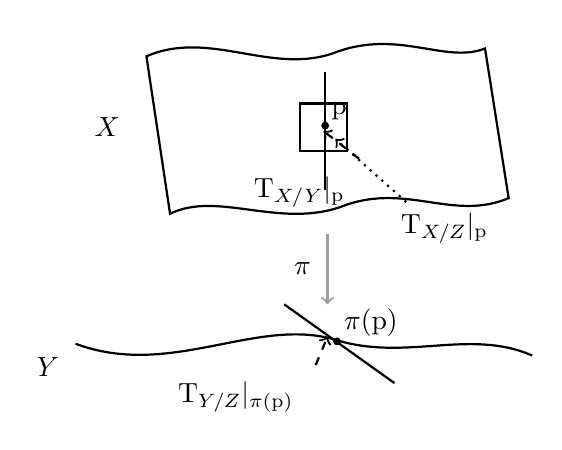
\begin{tikzpicture}[scale=1,line width=0.8pt]
  \draw (0.2,3.2) .. controls (1.0,3.55) and (1.8,2.95) .. (2.6,3.25)
        .. controls (3.4,3.55) and (4.0,3.1) .. (4.5,3.3)
        -- (4.8,1.4)
        .. controls (4.1,1.1) and (3.5,1.6) .. (2.7,1.3)
        .. controls (1.9,1.0) and (1.1,1.5) .. (0.5,1.2)
        -- cycle;
  \node at (-0.3,2.3) {$X$};
  \draw (2.15,2.0) rectangle (2.75,2.6);
  \draw (2.47,1.5) -- (2.47,3.0);
  \fill (2.47,2.32) circle (0.05);
  \node[anchor=south west,inner sep=1pt] at (2.5,2.35) {$\mathrm{p}$};
  \draw[dashed,->] (2.9,1.9) -- (2.45,2.25);
  \node[anchor=north east] at (2.85,1.8) {$\mathrm{T}_{X/Y}|_{\mathrm{p}}$};
  \draw[dotted,->] (3.5,1.35) -- (2.6,2.15);
  \node[anchor=north west] at (3.3,1.35) {$\mathrm{T}_{X/Z}|_{\mathrm{p}}$};
  \draw[->,gray!75] (2.5,0.95) -- (2.5,0.05);
  \node[anchor=east] at (2.42,0.5) {$\pi$};
  \draw (-0.7,-0.45) .. controls (0.5,-0.9) and (1.6,-0.1) .. (2.6,-0.4)
        .. controls (3.5,-0.68) and (4.3,-0.25) .. (5.1,-0.6);
  \draw (1.95,0.05) -- (3.35,-0.95);
  \fill (2.62,-0.42) circle (0.05);
  \node[anchor=south west,inner sep=1pt] at (2.66,-0.4) {$\pi(\mathrm{p})$};
  \node[anchor=north east] at (2.2,-0.8) {$\mathrm{T}_{Y/Z}|_{\pi(\mathrm{p})}$};
  \draw[dashed,->] (2.35,-0.72) -- (2.5,-0.36);
  \node at (-1.05,-0.75) {$Y$};
\end{tikzpicture}
\caption{余切正合列背后的几何。（依原书手绘图重绘。）}\label{fig:cotangent-exact-sequence-geometry}
\end{figure}

这份证明在代数上将相当直接，但这个陈述从根本上来自几何，而记住它的最好方式也正是几何。\cref{fig:cotangent-exact-sequence-geometry} 是一个映射 $\pi\colon X\to Y$ 的草图。这里 $X$ 应当理解为 $\Spec A$，$Y$ 理解为 $\Spec B$，而 $\Spec C$（我们马上会称之为 $Z$）是一个点。（如果你想要一幅 $\Spec C$ 维数更高的图，只须「把\cref{fig:cotangent-exact-sequence-geometry}与一条曲线作积」。）在图中，$Y$ 是「光滑的」，而 $X$ 是「在 $Y$ 上光滑的」——这粗略地说就是所有\trFiber{}都光滑。设 $\mathrm{p}$ 是 $X$ 的一个点。那么 $\pi$ 在 $\mathrm{p}$ 处的\trFiber{}的切空间当然是一个子空间，含于 $X$ 的\trTotalSpace{}在 $\mathrm{p}$ 处的切空间之中。其\trCokernel{}自然就是 $Y$ 在 $\pi(\mathrm{p})$ 处的切空间的拉回。对每个 $\mathrm{p}$ 而言的这个短正合列，应当是 $X$ 上「相对\trTangentSheaf」某个短正合列的一部分：
\[
0\longrightarrow\mathscr{T}_{X/Y}\longrightarrow\mathscr{T}_{X/Z}\longrightarrow\pi^*\mathscr{T}_{Y/Z}\longrightarrow 0
\]
（我们将在 \S21.2.18 中正式定义「相对\trTangentSheaf」。）取对偶便得
\[
0\longrightarrow\pi^*\Omega_{Y/Z}\longrightarrow\Omega_{X/Z}\longrightarrow\Omega_{X/Y}\longrightarrow 0.
\]
这恰好就是\mbox{定理~21.2.9} 的陈述，只不过这里我们还有\trLeftExactness。这一出入是因为定理的陈述更为一般；我们将在\mbox{练习~21.2.S} 中看到，在「光滑」的情形，我们的确有\trLeftExactness。

\textbf{21.2.10.}\ \emph{耐人寻味的注记。}\quad 一如既往，每当你见到某个\trRightExact{}的东西，你就应当怀疑：理应存在某种（上）同调理论，使这个东西是一条\trLongExactSequence{}的末端。事实的确如此，而这条正合列涉及\emph{\trAndre--\trQuillen{}同调}（André--Quillen homology）（详见 [E, p.~386]）。你应当期望左边的下一项是对应于 $A/B$ 的一阶同调，从而特别地不涉及 $C$。于是，如果你已经怀疑在 $A/B$ 与 $B/C$ 都「光滑」（不管这是什么意思）的情形下\trLeftExactness{}成立——此时\cref{fig:cotangent-exact-sequence-geometry} 的直观适用——那么你应当进一步期望：所需的一切只是 $A/B$ 「光滑」，而这将蕴涵第一\trAndre--\trQuillen{}同调应为零。即便你并不确切知道这些词都是什么意思，你也\emph{完全}正确！你还会对\emph{余切复形}（cotangent complex）生出一种隐约的直觉。在「充分光滑」的情形下\trLeftExactness{}成立的例子，见\mbox{命题~21.4.2} 与\mbox{练习~21.2.S}。更一般的陈述见 [Stacks, tag 06B6]。关于此列中接下来两项的清晰讨论，另见 [Liu, Cor.~6.3.22] 与 [Liu, Prop.~6.3.11]：「余切正合列」「\trConormal{}正合列」……

\textbf{21.2.11.}\ \emph{\mbox{定理~21.2.9} 的证明（余切正合列，仿射版本）。}\quad 首先，注意 $\Omega_{A/C}\to\Omega_{A/B}$ 的满性是显然的，因为该映射由 $\mathrm{d}a\mapsto\mathrm{d}a$ 给出（其中 $a\in A$）。

其次，穿过中间项的复合显然是 $0$，因为这个复合由 $a\otimes\mathrm{d}b\mapsto a\mathrm{d}b\mapsto 0$ 给出。

最后，我们希望把 $\Omega_{A/B}$ 识别为 $A\otimes_B\Omega_{B/C}\to\Omega_{A/C}$ 的\trCokernel。$\Omega_{A/B}$ 与 $\Omega_{A/C}$ 恰好相同，只是我们带有额外的关系：对 $b\in B$，$\mathrm{d}b=0$。而这些恰好就是左边 $1\otimes\mathrm{d}b$ 的像。\hfill$\square$

\textbf{21.2.12.\ \trhTheorem（\trConormal{}正合列，仿射版本）。}\ ——\ \emph{设 $B$ 是一个 $C$-代数，$I$ 是 $B$ 的一个\trIdeal，而 $A=B/I$。那么存在 $A$-模的一个自然正合列}
\[
I/I^2\xrightarrow{\ \delta\ }A\otimes_B\Omega_{B/C}\xrightarrow{\ a\otimes\mathrm{d}b\mapsto a\,\mathrm{d}b\ }\Omega_{A/C}\longrightarrow 0.
\]
\emph{映射 $\delta$ 由 $i\mapsto 1\otimes\mathrm{d}i$ 给出，或者更形式化地，$1\otimes\mathrm{d}\colon B/I\otimes_B I\to B/I\otimes_B\Omega_{B/C}$。}

（你会认出映射 $A\otimes_B\Omega_{B/C}\to\Omega_{A/C}$，它来自余切正合列，即\mbox{定理~21.2.9}。映射 $\delta$ 的一个特例曾悄悄出现在\mbox{练习~21.2.F} 中。）这个证明是代数性的，所以其后的几何讨论或有助于澄清你究竟应当如何看待它。

\emph{证明。}\quad 我们将把 $\delta\colon I/I^2\to A\otimes_B\Omega_{B/C}$ 的\trCokernel{}与 $\Omega_{A/C}$ 识别起来。考虑 $A\otimes_B\Omega_{B/C}$。作为 $A$-模，它由 $\mathrm{d}b$（其中 $b\in B$）生成，且服从三种类型的关系：对 $c\in\phi(C)$，$\mathrm{d}c=0$（其中 $\phi\colon C\to B$ 描述了 $B$ 作为 $C$-代数的地位）、可加性，以及\trLeibniz{}法则。给定任何\emph{在 $B$ 中}成立的关系，该关系的 $\mathrm{d}$ 便为 $0$。

现在，$\Omega_{A/C}$ 的定义与之类似，只不过\emph{在 $A$ 中}有更多的关系；而这些恰好就是 $I\subset B$ 的元素。于是我们这样得到 $\Omega_{A/C}$：从 $A\otimes_B\Omega_{B/C}$ 出发，再添加额外的关系 $\mathrm{d}i$（其中 $i\in I$）。但这恰好就是 $\delta$ 的像！（务必看清：$\delta$ 的\trCokernel{}与 $\Omega_{A/C}$ 的这一识别，恰恰正是经由映射 $a\otimes\mathrm{d}b\mapsto a\,\mathrm{d}b$ 实现的。）\hfill$\square$

现在我们来给出\trConormal{}正合列的一个几何诠释，并特别地定义\trConormalSheaf／\trConormal{}层／\trConormal{}丛。

与余切正合列（\mbox{定理~21.2.9}）一样，\trConormal{}正合列从根本上关乎几何。为给出动机，考虑\cref{fig:conormal-exact-sequence-geometry} 的草图。在这幅草图中，一切都是「光滑的」，$X$ 是一维的，$Y$ 是二维的，$j$ 是含入映射 $j\colon X\hookrightarrow Y$\footnote{原书图~21.3 中 $X\to Y$ 的箭头标注作「$\pi$」，而正文明言含入映射为 $j\colon X\hookrightarrow Y$，疑当为「$j$」，兹照录原书。——译者注}，而 $Z$ 是一个点。那么在一点 $\mathrm{p}\in X$ 处，切空间 $\mathscr{T}_X|_{\mathrm{p}}$ 显然单射入 $Y$ 中 $j(\mathrm{p})$ 处的切空间，而其\trCokernel{}便是 $Y$ 中 $X$ 在 $\mathrm{p}$ 处的正规向量空间。这应当给出 $X$ 上诸丛的一个正合列：
\[
0\longrightarrow\mathscr{T}_X\longrightarrow j^*\mathscr{T}_Y\longrightarrow\mathscr{N}_{X/Y}\longrightarrow 0.
\]
取对偶便应当得到
\[
0\longrightarrow\mathscr{N}_{X/Y}^{\vee}\longrightarrow j^*\Omega_{Y/Z}\longrightarrow\Omega_{X/Z}\longrightarrow 0.
\]
这恰好就是定理陈述中出现的内容，只不过：（i）代数几何中的这条正合列不必是\trLeftExact{}的；以及（ii）我们见到的是 $I/I^2$，而非 $\mathscr{N}^{\vee}_{\Spec A/\Spec B}$。

\begin{figure}[htbp]
\centering
\begin{tikzpicture}[scale=1,line width=0.8pt]
  \draw (0.2,1.9) -- (1.0,0.3);
  \node at (-0.25,1.1) {$X$};
  \draw[->,gray] (1.6,1.1) -- (3.0,1.1);
  \node at (2.3,1.45) {$\pi$};
  \draw (3.3,0.1) rectangle (5.7,2.0);
  \draw (3.85,1.85) -- (4.75,0.25);
  \node at (5.35,1.65) {$Y$};
  \draw[->,gray] (4.5,-0.15) -- (4.5,-0.85);
  \fill (4.5,-1.1) circle (0.05);
  \node at (4.85,-1.1) {$Z$};
\end{tikzpicture}
\caption{\trConormal{}正合列背后的几何。（依原书手绘图重绘。）}\label{fig:conormal-exact-sequence-geometry}
\end{figure}

\textbf{21.2.13.}\quad 我们这样解决第一个问题（i）：期望\mbox{定理~21.2.12} 的序列在适当「光滑」的情形下\trLeftExact，而事实的确如此；见\mbox{定理~21.2.31} 与\mbox{注记~21.2.32}。（如果你喜欢\mbox{注记~21.2.10}，你或许能正确猜出好几件事。左边下一项应当是 $A/C$ 的第一\trAndre--\trQuillen{}同调，所以我们应当只需要 $A/C$ 光滑，而 $B$ 应当无关紧要。另外，若 $A=B/I$，那么我们应当期望：$I/I^2$ 就是 $A/B$ 的第一\trAndre--\trQuillen{}同调。）

\textbf{21.2.14.}\ \emph{\trConormalSheaf{}与\trConormal{}层。}\quad 我们这样解决第二个问题（ii）：\emph{宣告} $I/I^2$ 为\textbf{\trConormalSheaf}（conormal module），并将在\mbox{定义~21.2.15} 中把那个显然的类似物定义为\emph{\trConormal{}层}（conormal sheaf）。

这里有一些几何直观，说明我们为何会想把（与 $I/I^2$ 相伴的层）称作\trConormal{}层；它很可能会让你困惑，但也可能带来一点启发。首先，若 $\Spec A$ 是 $\Spec B$ 的一个\trClosedPoint，我们便期望\trConormal{}空间恰为余切空间。而确实，若 $A=B/\mathfrak{m}$，则\trZariski{}余切空间正是 $\mathfrak{m}/\mathfrak{m}^2$。（我们在 \S13.1 中便做过这一微妙的联系。）特别地，早晚会有一天，你会形成一种感觉，明白为何 $\mathbb{A}^2_k=\Spec k[x,y]$ 中原点处的\trConormal（＝余切）空间自然地就是由线性形式 $\alpha x+\beta y$ 构成的空间。但接着考虑 $\Spec k[x,y,z]=\mathbb{A}^3_k$ 中由 $I=(x,y)$ 切出的 $z$-轴。$I/I^2$ 的元素可以写成 $\alpha(z)x+\beta(z)y$，其中 $\alpha(z)$ 与 $\beta(z)$ 是多项式。这就颇有理由应当是 $z$-轴的\trConormal{}空间：当 $z$ 变动时，$x$ 与 $y$ 的系数也随之变动。更一般地，同样的想法提示：$n$-空间内部任何坐标 $k$-平面的\trConormalSheaf／\trConormal{}层都对应于 $I/I^2$。现在考虑 $n$ 维\trManifold{} $Y$ 内部的一个 $k$ 维\trManifold{} $X$，带经典拓扑。我们可以实施同一构造：若 $\mathscr{I}$ 是 $Y$ 中 $X$ 的\trIdealSheaf，则 $\mathscr{I}/\mathscr{I}^2$ 可以与\trConormal{}层（本质上是余正规\trVectorBundle）识别起来，因为解析局部地看，$X\hookrightarrow Y$ 可以与 $\mathbb{R}^k\hookrightarrow\mathbb{R}^n$ 识别。由于这个原因，你或许会希望：在代数几何中，若 $\Spec A\hookrightarrow\Spec B$ 是「光滑」之物含入「光滑」之物的包含映射，则 $I/I^2$ 应当是\trConormalSheaf（或者在应用函子 $\sim$ 之后，\trConormal{}层）。受此启发，我们把余正规定义为\emph{总是} $I/I^2$，然后注意它具有良好的性质（例如\mbox{定理~21.2.12}），但须当心：要动手做出诸如 \S21.2.7 中那样的例子，弄清当我们不处在「光滑」情形时它可能有什么出乎意料的行为。

\textbf{21.2.15.}\ \emph{\trhDefinition{}。}\quad 设 $i\colon X\hookrightarrow Y$ 是概形的一个由\trIdealSheaf{} $\mathscr{I}$ 切出的\trClosedEmbedding。把\textbf{闭嵌入的\trConormal{}层}（conormal sheaf for a closed embedding）定义为 $\mathscr{I}/\mathscr{I}^2$，记作 $\mathscr{N}^{\vee}_{X/Y}$。（拟凝聚理想层的乘积定义于\mbox{练习~15.6.E}。）重要：我们把 $\mathscr{N}^{\vee}_{X/Y}$ 诠释为 $X$ 上的一个拟凝聚层，\textbf{而非}（仅仅是）$Y$ 上的——务必弄明白我们为什么可以这样做。（\mbox{练习~17.1.E} 是一条理由，但它造成的迷惑恐怕比提供的帮助还多。）

把\textbf{正规层}（normal sheaf）定义为其对偶 $\mathscr{N}_{X/Y}:=\mathscr{H}om(\mathscr{N}^{\vee}_{X/Y},\OO_X)$。这个记号并不完美，因为它暗示 $\mathscr{N}$ 的对偶总是 $\mathscr{N}^{\vee}$，而这并不总成立：正如对 $A$-模那样，从模到其双对偶的自然态射并不总是同构。（使此事成立的模称为\textbf{自反的}（reflexive），但我们不会使用这个概念。）

若正规层是有限秩的\trLocallyFreeSheaf，则我们称与之相伴的\trVectorBundle{}为 $Y$ 中 $X$ 的\textbf{正规丛}（normal bundle）。

\textbf{21.2.I.（容易练习）}\quad 对概形的一个\emph{局部闭嵌入} $i\colon X\hookrightarrow Y$，定义\textbf{\trConormal{}层}（conormal sheaf）$\mathscr{N}^{\vee}_{X/Y}$（从而正规层 $\mathscr{N}_{X/Y}$ 也随之而定），它是 $X$ 上的一个拟凝聚层。（务必确认你的定义是良定义的！）

在正则嵌入这个良好的情形中，\trConormal{}层（从而正规层）是有限秩的\trLocallyFreeSheaf（或者更不形式化地说，是一个\trVectorBundle）。特别地，$\mathscr{N}$ 的对偶的确是 $\mathscr{N}^{\vee}$。作为热身，我们先处理重要的余维数 $1$ 情形。

\textbf{21.2.J.（练习：有效\trCartierDivisor{}的正规丛）}\quad 设 $D\subset X$ 是一个有效\trCartierDivisor（\S9.5.1）。证明：\trConormal{}层 $\mathscr{N}^{\vee}_{D/X}$ 是 $\OO(-D)|_D$（从而特别地是一个\trInvertibleSheaf），因而正规层是 $\OO(D)|_D$。这为我们先前在 \S15.6.2 中对有效\trCartierDivisor{}的正规丛所下之定义提供了理据。可能令人惊讶的是：当 $X\cong\mathbb{A}^2$ 而 $D$ 是两条坐标轴之并时（更一般地，当 $X$ 正则而 $D$\trSingular{}时），正规层竟然是局部自由的，因为你也许习惯了「\trTubularNeighborhood」（tubular neighborhood）同构于正规丛的想法。

现在我们来处理一般情形。

\textbf{21.2.16.\ \trhProposition。}\ ——
\emph{（a）若\trIdeal{} $I\subset B$ 由一个\trRegularSequence{} $x_1,\dots,x_r$ 生成，则由
\begin{equation*}\tag{21.2.16.1}\label{eq:regular-sequence-conormal}
(a_1,\dots,a_r)\longmapsto a_1x_1+\cdots+a_rx_r
\end{equation*}
给出的映射 $\gamma\colon(B/I)^{\oplus r}\to I/I^2$ 是一个同构，从而把 $I/I^2$ 描述为 $B/I$ 上秩 $r$ 的自由模、以 $x_1,\dots,x_r$ 为基。
（b）余维数为 $r$ 的正则嵌入的（余）正规层是秩 $r$ 的局部自由层。}

（不需要任何\trNoetherian{}假设。）\mbox{练习~24.6.D} 在「$A$ 包含一个域」这一常用情形中给出了（b）的一个不同的、简短的证明（如果你留心的话，其实（a）也在其内）。

\emph{证明。}\quad（a）显然 \eqref{eq:regular-sequence-conormal} 是满的，所以我们只须证明单性。设 $b_1,\dots,b_r\in B$ 满足 $b_1x_1+\cdots+b_rx_r\in I^2$；我们希望证明 $b_i\in I$ 对一切 $i$ 成立。这是下面两个陈述（$a_k$）与（$b_k$）（二者都取 $1\le k\le r$）的推论。

（$a_k$）：设 $b_1,\dots,b_k\in B$ 满足
\begin{equation*}\tag{21.2.16.2}\label{eq:ak-hypothesis}
b_1x_1+\cdots+b_kx_k\in(x_1,\dots,x_k)^2,
\end{equation*}
则 $b_k\in(x_1,\dots,x_k)$。

（$b_k$）：设 $b_1,\dots,b_{k-1}\in B$ 满足
\begin{equation*}\tag{21.2.16.3}\label{eq:bk-hypothesis}
b_1x_1+\cdots+b_{k-1}x_{k-1}\in(x_1,\dots,x_k)^2,
\end{equation*}
则存在 $d_1,\dots,d_{k-1}\in B$ 使得
\begin{equation*}\tag{21.2.16.4}\label{eq:bk-conclusion}
(b_1-d_1x_k)x_1+\cdots+(b_{k-1}-d_{k-1}x_k)x_{k-1}\in(x_1,\dots,x_{k-1})^2.
\end{equation*}

我们先证（$a_k$）。模去 $(x_1,\dots,x_{k-1})$，\eqref{eq:ak-hypothesis} 就变成 $b_kx_k\in(x_k^2)$。于是（由于依\trRegularSequence{}的定义，$x_k$ 是模 $(x_1,\dots,x_{k-1})$ 意义下的非\trZerodivisor），$b_k$ 在模 $(x_1,\dots,x_{k-1})$ 意义下是 $x_k$ 的倍数，故 $b_k\in(x_1,\dots,x_k)$，正如所愿。

我们接着证（$b_k$）。此时 \eqref{eq:bk-hypothesis} 蕴涵
\[
b_1x_1+\cdots+b_{k-1}x_{k-1}=C+(c_1x_1+\cdots+c_kx_k)x_k
\]
对某些 $c_i\in B$ 与某个 $C\in(x_1,\dots,x_{k-1})^2$ 成立。于是 $0\equiv(c_1x_1+\cdots+c_kx_k)x_k$（模 $(x_1,\dots,x_{k-1})$）。由于 $x_k$ 不是模 $(x_1,\dots,x_{k-1})$ 意义下的\trZerodivisor，我们有
\[
c_1x_1+\cdots+c_kx_k=d_1x_1+\cdots+d_{k-1}x_{k-1}
\]
对某些 $d_1,\dots,d_{k-1}\in B$ 成立。于是
\[
(b_1-d_1x_k)x_1+\cdots+(b_{k-1}-d_{k-1}x_k)x_{k-1}=C\in(x_1,\dots,x_{k-1})^2,
\]
这就给出了 \eqref{eq:bk-conclusion}，正如所愿。

（b）由（a）立得。\hfill$\square$

我们很快会遇到一个相关但更难的事实：若 $\mathscr{I}$ 是一个余维数为 $r$ 的正则嵌入的理想层，则 $\mathscr{I}^n/\mathscr{I}^{n+1}$ 局部自由，因为它就是 $\Sym^n(\mathscr{I}/\mathscr{I}^2)$（\mbox{推论~22.3.9}，或\mbox{练习~24.6.E}）。

\textbf{21.2.17. 第二个定义：\trUniversalProperty。}\quad 这是第二个定义，它在哲理上很重要，以\trUniversalProperty{}给出。当然，这是一个刻画而非定义：凭泛性质式的几句废话，它表明若该模（连同映射 $\mathrm{d}$）存在，则它在相差唯一\trIsomorphism{}的意义下唯一；而此后你仍然需要动手构造它，以确信它存在。

设 $A$ 是一个 $B$-代数，而 $M$ 是一个 $A$-模。\textbf{$A$ 到 $M$ 的 $B$-线性\trDerivation}（$B$-linear derivation of $A$ into $M$）是 $B$-模的一个映射 $\mathrm{d}\colon A\to M$（\emph{不必是} $A$-模的映射），满足\trLeibniz{}法则：$\mathrm{d}(fg)=f\,\mathrm{d}g+g\,\mathrm{d}f$。举一例：设 $B=k$、$A=k[x]$、$M=A$，则 $\mathrm{d}/\mathrm{d}x$ 是一个 $k$-线性\trDerivation。再举一例：若 $B=k$、$A=k[x]$、$M=k$，则 $(\mathrm{d}/\mathrm{d}x)|_0$（「在 $0$ 处取导数值」这一算子）是一个 $k$-线性\trDerivation。

第三个例子是 $\mathrm{d}\colon A\to\Omega_{A/B}$，而且事实上 $\mathrm{d}\colon A\to\Omega_{A/B}$ 就是\emph{$A$ 的泛 $B$-线性\trDerivation}。确切地说，映射 $\mathrm{d}\colon A\to\Omega_{A/B}$ 由下面的\trUniversalProperty{}定义：任何其他 $B$-线性\trDerivation{} $\mathrm{d}'\colon A\to M$ 都唯一地穿过 $\mathrm{d}$：
\begin{tikzcd}
A\ar[rr,"\mathrm{d}'"]\ar[dr,"\mathrm{d}"'] && M\\
& \Omega_{A/B}\ar[ur,"f"']
\end{tikzcd}
其中 $f$ 是 $A$-模的一个映射。（再次注意：$\mathrm{d}$ 与 $\mathrm{d}'$ 未必是 $A$-模的映射——它们只是 $B$-线性的。）凭泛性质式的几句废话，若它存在，便在相差唯一\trIsomorphism{}的意义下唯一。映射 $\mathrm{d}\colon A\to\Omega_{A/B}$ 显然满足这条\trUniversalProperty，基本上就是按定义。

取决于你的大脑如何运转，做接下来两道练习时，你可能更愿意使用第一个（构造性的）定义或第二个（\trUniversalProperty{}式的）定义。

\textbf{21.2.K.（练习）}

（a）\emph{（\trDifferential{}的拉回）}\ 若
\begin{tikzcd}
A' & A\ar[l]\\
B'\ar[u] & B\ar[l]\ar[u]
\end{tikzcd}
是一个交换图表，请描述 $A'$-模的一个自然\trHomomorphism{} $A'\otimes_A\Omega_{A/B}\to\Omega_{A'/B'}$。一个重要的特例是 $B=B'$。

（b）\emph{（\trDifferential{}对基扩张表现良好，仿射情形）}\quad 再若上面的图表是一个「张量图表」（即 $A'\cong B'\otimes_B A$，从而该图表是「余笛卡儿」的（co-Cartesian）），证明 $A'\otimes_A\Omega_{A/B}\to\Omega_{A'/B'}$ 是一个同构。（视你的进路而定，这可能比你预期的更刁钻。）

\textbf{21.2.L.（练习：\trLocalization{}（加强版；较\mbox{例~21.2.8}））}\quad 设 $\phi\colon B\to A$ 是环的一个映射，$S$ 是 $A$ 的一个\trMultiplicativeSubset，$T$ 是 $B$ 的一个\trMultiplicativeSubset{}且 $\phi(T)\subset S$，于是我们有下面的交换图表。
\begin{tikzcd}
S^{-1}A & A\ar[l]\\
T^{-1}B\ar[u] & B\ar[l]\ar[u]
\end{tikzcd}
证明：\mbox{练习~21.2.K(a)} 的\trDifferential{}之拉回 $S^{-1}\Omega_{A/B}\to\Omega_{S^{-1}A/T^{-1}B}$ 是一个同构。（从「相对\trTangentVector」的直观图像看，这应当是可信的。）一个重要情形是 $T=\{1\}$。

\textbf{21.2.M.（练习：域扩张（续）；较\mbox{练习~21.2.H}）}

（a）计算 $\Omega_{K(t)/k}$。（提示：先用 \S21.2.6，接\mbox{练习~21.2.L}。）

（b）若 $K/k$ 由 $t_1,\dots,t_n\in K$ \emph{\trSeparablyGenerated}（也就是说，$t_1,\dots,t_n$ 构成一个\trTranscendenceBase，而 $K/k(t_1,\dots,t_n)$ 是代数且可分的，\S10.5.18），证明：$\Omega_{K/k}$ 是一个自由 $K$-模（即\trVectorSpace），以 $\mathrm{d}t_1,\dots,\mathrm{d}t_n$ 为基。一条可行的进路：对 $k\hookrightarrow k(t_1,\dots,t_n)\hookrightarrow K$ 用余切正合列（\mbox{定理~21.2.9}），证明诸 $\mathrm{d}t_i$ 张成作为 $K$-\trVectorSpace{}的 $\Omega_{K/k}$。棘手之处在于证明诸 $\mathrm{d}t_i$ 线性无关。做法是：证明存在唯一的映射 $\Omega_{K/k}\to K$，把 $\mathrm{d}t_1$ 送到 $1$，而把 $\mathrm{d}t_i$（$i>1$）送到 $0$。先就 $K/k(t_1,\dots,t_n)$ 由单个元素生成的情形做出来；再做有限生成的情形；至于一般情形，则通过在一切有限生成子扩张上定义该映射、并借唯一性证明它们「彼此全相合」来完成。

\textbf{21.2.18. 第三个定义：整体化。}\quad 现在我们想把上述定义对概形的任意态射 $\pi\colon X\to Y$ 整体化。我们可以「逐个仿射地」做这件事；只须确保上面的概念对「仿射集的更换」表现良好。这样，$X$ 上的一支相对\trDifferential{}将是如下数据：对每个仿射 $\mathrm{U}\subset X$，给定一支形如 $\sum a_i\,\mathrm{d}b_i$ 的\trDifferential，而在两个仿射\trOpenSet{}的交 $\mathrm{U}\cap\mathrm{U}'$ 上，给定的两支\trDifferential{}分别以 $\mathrm{U}$ 上的 $\sum a_i\,\mathrm{d}b_i$ 与 $\mathrm{U}'$ 上的 $\sum a'_i\,\mathrm{d}b'_i$ 为代表元，且二者在交叠处相等。不过我们不走这条路，而是换一种做法。我会先给出（看似反直观的）定义，然后告诉你应当如何思考它，最后再回到定义本身。

设 $\pi\colon X\to Y$ 是概形的任意态射。回忆 $\delta\colon X\to X\times_YX$ 是一个局部闭嵌入（\mbox{命题~11.2.1(b)}）。\emph{定义}\textbf{相对\trCotangentSheaf}（relative cotangent sheaf）$\Omega_{X/Y}$（或 $\Omega_\pi$）为对角线的\trConormal{}层 $\mathscr{N}^{\vee}_{X/X\times_YX}$（见 \S21.2.14——而若 $X\to Y$ 是\trSeparated{}的，你甚至无须为\mbox{练习~21.2.I} 担心）。（眼下也是定义\textbf{相对\trTangentSheaf}（relative tangent sheaf）$\mathscr{T}_{X/Y}$ 的好时机：取相对\trCotangentSheaf{}的对偶 $\mathscr{H}om(\Omega_{X/Y},\OO_X)$。若我们在 $k$-概形的范畴中工作，则 $\Omega_{X/k}$ 与 $\mathscr{T}_{X/k}$ 常分别称作 $X$ 的\textbf{\trCotangentSheaf}（cotangent sheaf）与\textbf{\trTangentSheaf}（tangent sheaf）。）

现在我们来定义 $\mathrm{d}\colon\OO_X\to\Omega_{X/Y}$。令 $\mathrm{pr}_1\colon X\times_YX\to X$ 与 $\mathrm{pr}_2\colon X\times_YX\to X$ 为那两个\trProjection。于是在\trOpenSet{} $\mathrm{U}$ 上如下定义 $\mathrm{d}\colon\OO_X\to\Omega_{X/Y}$：
\[
\mathrm{d}f=\mathrm{pr}_2^*f-\mathrm{pr}_1^*f.
\]
（你该如何把 $\mathrm{pr}_2^*f-\mathrm{pr}_1^*f$ 诠释为 $\Omega_{X/Y}$ 的一个\trSection？）

\emph{警告}：$\mathrm{d}$ 不是 $X$ 上诸拟凝聚层之间的态射，尽管按这句话唯一可能有的含义，它\emph{是} $\OO_Y$-线性的。

我们很快会看到：$\mathrm{d}$ 的确是层 $\OO_X$ 的一个\trDerivation（按这句话唯一可能有的含义），同时还会看到，我们的新\trDifferential{}概念在仿射\trOpenSet{}上与旧定义相合，从而把定义整体化了。注意，对任意\trOpenSubset{} $\mathrm{U}\subset X$，$\mathrm{d}$ 诱导出一个映射
\begin{equation*}\tag{21.2.18.1}\label{eq:global-d-sections}
\Gamma(\mathrm{U},\OO_X)\longrightarrow\Gamma(\mathrm{U},\Omega_{X/Y}),
\end{equation*}
我们也称之为 $\mathrm{d}$，并把它诠释为「求导」。

\textbf{21.2.19.}\ \emph{动机。}\quad 在把它与其余几个定义联系起来之前，请先让我试着说服你：这是一个合理的定义。（这段讨论是非形式的、不严格的。）比如说，$Y$ 是一个点，而 $X$ 是一个\trManifold。那么 $X\times X$ 上的\trTangentBundle{} $\mathrm{T}_{X\times X}$ 是 $\mathrm{pr}_1^*\mathrm{T}_X\oplus\mathrm{pr}_2^*\mathrm{T}_X$，其中 $\mathrm{pr}_1$ 与 $\mathrm{pr}_2$ 是从 $X\times X$ 到它的两个因子的\trProjection。把它限制到对角线 $\Delta$ 上，并考察正规丛正合列：
\[
0\longrightarrow\mathrm{T}_\Delta\longrightarrow\mathrm{T}_{X\times X}|_\Delta\longrightarrow\mathscr{N}_{\Delta/X}\longrightarrow 0.
\]
现在，左边的态射把 $v$ 送到 $(v,v)$，于是其\trCokernel{}可以诠释为 $(v,-v)$。这样一来，$\mathscr{N}_{\Delta/X}$ 同构于 $\mathrm{T}_X$。于是我们可以反其道而行：我们知道怎样找出\trNormalBundle{}（或者更精确地说，\trConormal{}层），而我们就可以用它来定义\trTangentBundle{}（或者更精确地说，\trCotangentSheaf）。

\textbf{21.2.20.}\ \emph{再谈动机。}\quad 如果你动手做过\mbox{扩展例题~15.3.4}，你或许会发现这里的许多想法在那里已隐约可见，例如 $\mathrm{pr}_2^*f-\mathrm{pr}_1^*f$，以及在「对角线的理想、模去其平方」之中工作。

\textbf{21.2.21.}\ \emph{在仿射情形中检验。}\quad 现在我们来看看，对于 $\Spec A\to\Spec B$ 这一特殊情形，这一切是如何运作的。此时对角态射 $\delta\colon\Spec A\hookrightarrow\Spec A\otimes_BA$ 对应于 $A\otimes_BA$ 的理想 $I$，它是环映射
\[
\alpha\colon\sum x_i\otimes y_i\longmapsto\sum x_iy_i
\]
的\trKernel。

\textbf{21.2.22.}\quad $A\otimes_BA$ 的理想 $I$ 由形如 $1\otimes a-a\otimes 1$ 的元素生成。理由：若 $\alpha(\sum x_i\otimes y_i)=0$，即 $\sum x_iy_i=0$，则
\[
\sum x_i\otimes y_i=\sum(x_i\otimes y_i-x_iy_i\otimes 1)=\sum(x_i\otimes 1)(1\otimes y_i-y_i\otimes 1).
\]

这个\trDerivation{}是 $\mathrm{d}\colon A\to A\otimes_BA$，$a\mapsto(1\otimes a-a\otimes 1)$（这是 $I$ 的一个元素，取模 $I^2$ 后看待）。（在验证它与我们先前的定义相合之前，我们实在不该把它称作「$\mathrm{d}$」，但我们还是不负责任地就这么叫了。）

我们来检验 $\mathrm{d}$ 的确是一个\trDerivation（\S21.2.17）。显然 $\mathrm{d}$ 是 $B$-线性的，所以我们检验\trLeibniz{}法则：
\begin{align*}
\mathrm{d}(aa')-a\,\mathrm{d}a'-a'\,\mathrm{d}a &= 1\otimes aa'-aa'\otimes 1-a\otimes a'+aa'\otimes 1-a'\otimes a+a'a\otimes 1\\
&= -a\otimes a'-a'\otimes a+a'a\otimes 1+1\otimes aa'\\
&= (1\otimes a-a\otimes 1)(1\otimes a'-a'\otimes 1)\\
&\in I^2.
\end{align*}
于是，由 $\Omega_{A/B}$ 的\trUniversalProperty，我们有 $A$-模的一个自然态射 $\Omega_{A/B}\to I/I^2$。

\textbf{21.2.23.\ \trhTheorem。}\ ——\ \emph{由 $\Omega_{A/B}$ 的\trUniversalProperty{}诱导的自然态射 $f\colon\Omega_{A/B}\to I/I^2$ 是一个同构。}

\emph{证明。}\quad 我们将按如下路线证明。（i）我们将证明 $f$ 是满的，而（ii）我们将描述 $g\colon I/I^2\to\Omega_{A/B}$，使得 $g\circ f\colon\Omega_{A/B}\to\Omega_{A/B}$ 是恒等映射（从而表明 $f$ 是单的）。

（i）映射 $f$ 把 $\mathrm{d}a$ 送到 $1\otimes a-a\otimes 1$，而这类元素生成 $I$（\S21.2.22），故 $f$ 是满的。

（ii）考虑由 $x\otimes y\mapsto x\,\mathrm{d}y$ 定义的映射 $A\otimes_BA\to\Omega_{A/B}$。（由 $\otimes$ 的\trUniversalProperty，这是一个良定义的映射；见 \S1.2.5。）把 $g\colon I/I^2\to\Omega_{A/B}$ 定义为该映射到 $I$ 上的限制。我们须检验这是良定义的，也就是说，$I^2$ 的元素都被送到 $0$，换言之，我们需要：
\[
\Bigl(\sum x_i\otimes y_i\Bigr)\Bigl(\sum x'_j\otimes y'_j\Bigr)=\sum_{i,j}x_ix'_j\otimes y_iy'_j\longmapsto 0
\]
其中 $\sum_i x_iy_i=\sum_j x'_jy'_j=0$。但由\trLeibniz{}法则，
\begin{align*}
\sum_{i,j}x_ix'_j\,\mathrm{d}(y_iy'_j) &= \sum_{i,j}x_ix'_jy_i\,\mathrm{d}y'_j+\sum_{i,j}x_ix'_jy'_j\,\mathrm{d}y_i\\
&= \biggl(\sum_i x_iy_i\biggr)\biggl(\sum_j x'_j\,\mathrm{d}y'_j\biggr)+\biggl(\sum_i x_i\,\mathrm{d}y_i\biggr)\biggl(\sum_j x'_jy'_j\biggr)\\
&= 0.
\end{align*}
于是 $g\circ f$ 的确是恒等映射，因为
\[
\mathrm{d}a\xrightarrow{\ f\ }1\otimes a-a\otimes 1\xrightarrow{\ g\ }1\,\mathrm{d}a-a\,\mathrm{d}1=\mathrm{d}a,
\]
正如所愿。\hfill$\square$

\textbf{21.2.N.（容易练习）}\quad 设 $\pi\colon X\to Y$ 是概形的一个态射，带有开子概形 $\Spec A\subset X$ 与 $\Spec B\subset Y$，且 $\Spec A\subset\pi^{-1}(\Spec B)$。把 $\Omega_{X/Y}|_{\Spec A}$ 与 $\widetilde{\Omega}_{A/B}$ 识别起来，并把 $\mathrm{d}\colon\Gamma(\Spec A,\OO_X)\to\Gamma(\Spec A,\Omega_{X/Y})$ 与 $\mathrm{d}\colon A\to\Omega_{A/B}$ 识别起来。于是，整体构造的确自然地把仿射构造「黏合起来」。

现在我们可以利用「$\Omega$ 在仿射\trOpenSet{}上如何运作」的理解，把先前的诸陈述推广到非仿射的场合。

\textbf{21.2.O.（练习）}\quad 若 $\mathrm{U}\subset X$ 是一个\trOpenSubset，证明：映射 \eqref{eq:global-d-sections} 是一个\trDerivation。

\textbf{21.2.P.（练习）}\quad 设 $\pi\colon X\to Y$ 局部有限型，而 $Y$（从而 $X$）局部\trNoetherian。证明：$\Omega_{X/Y}$ 是 $X$ 上的一个凝聚层。（不妨放松\trNoetherian{}假设以换取较弱的结论。）

\textbf{21.2.Q.（练习）}\quad 设 $\pi\colon X\to Y$ 相对维数 $n$ \trSmooth。证明：$\Omega_{X/Y}$ 是秩 $n$ 的局部自由层。提示：$\Omega$ 的\trJacobianMatrix{}式描述，即\mbox{练习~21.2.E}。

概形的余切正合列与\trConormal{}正合列现在便可直接得出。

\textbf{21.2.24.\ \trhTheorem。}\ ——
\emph{（a）（余切正合列）设}
\begin{tikzcd}
X\ar[r,"\pi"] & Y\ar[r,"\rho"] & Z
\end{tikzcd}
\emph{是概形的态射。那么存在 $X$ 上拟凝聚层的一个正合列}
\[
\pi^*\Omega_{Y/Z}\longrightarrow\Omega_{X/Z}\longrightarrow\Omega_{X/Y}\longrightarrow 0,
\]
\emph{此即\mbox{定理~21.2.9} 的整体化。
（b）（\trConormal{}正合列）设 $\rho\colon Y\to Z$ 是概形的一个态射，而 $\iota\colon X\hookrightarrow Y$ 是一个闭嵌入，带\trConormal{}层 $\mathscr{N}^{\vee}_{X/Y}$。那么存在 $X$ 上拟凝聚层的一个正合列}
\[
\mathscr{N}^{\vee}_{X/Y}\xrightarrow{\ \delta\ }\iota^*\Omega_{Y/Z}\longrightarrow\Omega_{X/Z}\longrightarrow 0,
\]
\emph{此即\mbox{定理~21.2.12} 的整体化。}

\textbf{21.2.R.（练习）}\quad 证明\mbox{定理~21.2.24}。（哪些地方需要检验？）

你应当期望：在适当的光滑性之下，这些正合列也同样左正合（见\mbox{注记~21.2.10} 与 \S21.2.13）。下面的结果是余切正合列的一个重要特例。（\mbox{定理~21.2.31} 将对光滑簇的\trConormal{}正合列给出一个类似的陈述。）

\textbf{21.2.S.（练习：$\pi$ 与 $\rho$ 光滑时余切正合列的左正合性）}\quad 证明：若 $\pi$ 与 $\rho$ 都光滑，则余切正合列左正合。提示：你在\mbox{练习~13.6.D} 中用过的那个 $(m+n)\times(m+n)$ 矩阵是「块上三角」的。

\textbf{21.2.25.}\ \emph{拉回相对微分。}\quad 不出所料，相对微分层可以拉回，并且它在\trBaseChange{}下表现良好。

\textbf{21.2.26.\ \trhTheorem（微分的拉回）。}\ ——
\emph{（a）若}
\begin{tikzcd}
X'\ar[r,"\mu"]\ar[d] & X\ar[d]\\
Y'\ar[r] & Y
\end{tikzcd}
\emph{是概形的一个交换图表，则存在 $X'$ 上拟凝聚层的一个自然\trHomomorphism{} $\mu^*\Omega_{X/Y}\to\Omega_{X'/Y'}$。一个重要的特例是 $Y=Y'$。}
\emph{（b）（$\Omega$ 在\trBaseChange{}下表现良好）再若上面的图表是一个笛卡儿方格（从而 $X'\cong X\times_YY'$），则 $\mu^*\Omega_{X/Y}\to\Omega_{X'/Y'}$ 是一个同构。}

\textbf{21.2.T.（练习）}\quad 由\mbox{练习~21.2.K} 推出\mbox{定理~21.2.26}。（为什么\mbox{练习~21.2.K(a)} 的构造「黏合良好」？）

作为\mbox{定理~21.2.26(b)} 的一个特别情形，相对微分层的\trFiber{}的确就是该\trFiber{}的微分层。这样一来，「微分层」这一概念的确把每支\trFiber{}上的微分「黏合起来」了。

\textbf{21.2.U.（练习）}\quad 设 $\alpha\colon X\to Z$ 与 $\beta\colon Y\to Z$ 是两个态射，而 $\alpha'\colon X\times_ZY\to Y$ 与 $\beta'\colon X\times_ZY\to X$ 是由纤维积诱导的态射。描述一个同构
\[
\Omega_{X\times_ZY/Z}\overset{\sim}{\longleftrightarrow}(\beta')^*\Omega_{X/Z}\oplus(\alpha')^*\Omega_{Y/Z}.
\]
（右边常写作 $\Omega_{X/Z}\boxplus\Omega_{Y/Z}$。）

\textbf{21.2.27. 重要：重访簇的光滑性。}

设 $k$ 是一个域。自 \S13.2.3 以来，我们一直在使用一个颇为别扭的 $k$-光滑性定义，而现在我们要把 $k$-光滑性的定义锻造得更稳健一些。

\textbf{21.2.28.}\ \emph{重新定义。}\quad 若一个 $k$-概形 $X$ 局部有限型、纯维数为 $n$，且 $\Omega_{X/k}$ 是秩 $n$ 的局部自由层，则称它是\textbf{维数 $n$ 的 $k$-光滑}（$k$-smooth of dimension $n$）或\textbf{在 $k$ 上维数 $n$ 光滑}（smooth of dimension $n$ over $k$）的。维数 $n$ 常被省去，而人们可能（也许）会想把某种东西称作光滑的——倘若它是各种维数的光滑之物的（概形论）不交并。

\textbf{21.2.V.（练习）}\quad 证明：\mbox{重新定义~21.2.28} 的 $k$-光滑性与\mbox{定义~13.2.4} 相合。（提示：二者都可以用\trJacobianMatrix{}的\trCokernel{}来描述。）

\textbf{21.2.29.}\ \emph{注记。}\quad 不要多久，我们还将在\mbox{定理~24.8.8} 中重访光滑态射的定义（\mbox{定义~13.6.2}）。

\textbf{21.2.W.}\ \extrahard\ \textbf{（练习：给有复几何背景的读者）}\quad 设 $X$ 是一个复代数\trVariety。证明：$X$ 的解析化 $X^{\mathrm{an}}$（定义于\mbox{练习~7.3.P}）光滑（在微分几何的意义下），当且仅当 $X$ 光滑（在代数几何的意义下，即在 $\mathbb{C}$ 上）。此时，证明复流形 $X^{\mathrm{an}}$ 的复维数（即实维数的一半）是 $\dim X$。提示：\trJacobianCriterion{}在两种场合都适用。

\textbf{21.2.30. 光滑簇之嵌入的\trConormal{}正合列的左正合性。}

正如 \S21.2.13 中所描述的，我们期望\trConormal{}正合列在适当「光滑」的情形下左正合。

\textbf{21.2.31.\ \trhTheorem（光滑簇的\trConormal{}正合列）。}\ ——\ \emph{设 $\iota\colon X\hookrightarrow Y$ 是域 $k$ 上光滑簇的一个闭嵌入，带\trConormal{}层 $\mathscr{N}^{\vee}_{X/Y}$。那么 $\mathscr{N}^{\vee}_{X/Y}$ 局部自由，而\trConormal{}正合列（\mbox{定理~21.2.24(b)}）左正合：}
\begin{equation*}\tag{21.2.31.1}\label{eq:conormal-smooth-left-exact}
0\longrightarrow\mathscr{N}^{\vee}_{X/Y}\xrightarrow{\ \delta\ }\iota^*\Omega_{Y/k}\longrightarrow\Omega_{X/k}\longrightarrow 0
\end{equation*}
\emph{正合。}

取对偶，即应用 $\mathscr{H}om(\cdot,\OO_X)$，我们便得到\textbf{正规正合列}（normal exact sequence）
\[
0\longrightarrow\mathscr{T}_{X/k}\longrightarrow\mathscr{T}_{Y/k}|_X\longrightarrow\mathscr{N}_{X/Y}\longrightarrow 0
\]
（其正合性由\mbox{练习~14.2.I} 保证），而它在几何上更为直观（见\cref{fig:conormal-exact-sequence-geometry} 与\mbox{定理~21.2.12} 证明之后的讨论）。

\textbf{21.2.32.}\ \emph{注记。}\quad 余正规列在更为一般的情形下也左正合。基本上所需要的一切，只是 $\iota\circ g\colon X\to Z$ 的适当光滑性\footnote{原书此处作「$\iota\circ g\colon X\to Z$」，然而按上下文 $g$ 未曾定义，疑当为「$g\circ\iota$」（即 \mbox{定理~21.2.24(b)} 中 $Y\to Z$ 与闭嵌入 $\iota$ 的复合 $X\to Z$）之误，兹照录原书。——译者注}；相关事实见 [Stacks, tag 06B7] 与 [Stacks, tag 06BB]。特别地，$Y$ 的光滑性无关紧要！由此，下面的\mbox{重要推论~21.2.33} 对一般的有限型 $Y$ 也成立。

\emph{证明。}

\textbf{21.2.X.（练习）}\quad 证明：\mbox{定理~21.2.31} 为真，当且仅当它经\trBaseChange{}到 $k$ 的代数闭包 $\bar{k}$ 后为真。提示：证明 \eqref{eq:conormal-smooth-left-exact} 中所有项的构造都与代数域扩张相安无事。\trDifferential{}的情形见\mbox{定理~21.2.26}；\trConormal{}层的情形，则请检验其定义与代数域扩张相安无事。

于是我们可以假定 $k$ 代数闭，从而（由\mbox{练习~13.2.J}）光滑 $k$-概形的\trClosedPoint{}都正则。设 $\mathscr{I}$ 为 $\iota\colon X\hookrightarrow Y$ 的\trIdealSheaf。对任一\trClosedPoint{} $\mathrm{p}\in X$，由\mbox{练习~13.2.M(b)}，$\iota$ 在 $\mathrm{p}$ 的一个开邻域内是正则嵌入。因此 $\iota$ 是正则嵌入。（你明白为什么吗？）于是由\mbox{命题~21.2.16(b)}，$\mathscr{I}/\mathscr{I}^2$ 是秩 $r$ 的局部自由层。由\mbox{练习~6.6.G(a)}，$\ker\delta$ 的诸\trAssociatedPoint{}是 $\mathscr{I}/\mathscr{I}^2$ 的诸\trAssociatedPoint{}的一个子集，所以要证 $\ker\delta=0$，只须在 $\mathscr{I}/\mathscr{I}^2$ 的诸\trAssociatedPoint{}处检验，而这些恰恰就是 $X$ 的诸\trAssociatedPoint（因为 $\mathscr{I}/\mathscr{I}^2$ 局部自由）。

由\mbox{命题~13.2.13}（光滑蕴涵既约），$X$ \trReduced。于是我们只须在 $X$（的诸\trIrreducibleComponent）的诸\trGenericPoint{}处检验（因为 $X$ 没有内嵌点；见 \S6.6.2 或\mbox{练习~6.6.R}）。但这要检验一个右正合的\trVectorSpace{}列的\trLeftExactness（$X$ 既约保证了在\trGenericPoint{}处的茎是\trVectorSpace），而由于左边的维数（即 $X$ 在 $Y$ 中的余维数，由\mbox{命题~21.2.16(b)} 给出）恰是另外两者之差，我们就做完了。\hfill$\square$

\textbf{21.2.33. 重要推论。}\ ——\ \emph{设 $Y$ 是一个光滑 $k$-\trVariety，而 $\mathrm{q}\in Y$ 是一个剩余域 $\kappa(\mathrm{q})$ 在 $k$ 上可分的\trClosedPoint。（若 $\operatorname{char}k=0$ 或 $k$ 是有限域，则自动如此。）那么 $\mathrm{q}\hookrightarrow Y$ 的\trConormal{}正合列给出：$Y$ 在 $\mathrm{q}$ 处的\trZariski{}\trCotangentSpace{}与 $\Omega_{Y/k}$ 在 $\mathrm{q}$ 处的\trFiber{}之间的一个同构。}

\emph{证明。}\quad 对 $X=\mathrm{q}$ 应用\mbox{定理~21.2.31}。注意 $\mathrm{q}$ 的确是一个光滑 $k$-\trVariety（用 $\kappa(\mathrm{q})/k$ 的可分性！），而且 $\Omega_{\mathrm{q}/k}=0$。\hfill$\square$

\textbf{21.2.34.}\ \emph{注记。}\quad 若 $Y$ 光滑，这个结果便把\mbox{练习~21.2.F} 推广到了可分闭点；而且如\mbox{注记~21.2.32} 中所述，就连 $Y$ 的这个光滑性条件也可以去掉。正如\mbox{练习~21.2.F} 的陈述之后所描述的，这有一系列推论。例如，它把\trZariski{}切空间的\trJacobianMatrix{}式描述延拓到了可分闭点。

\textbf{21.2.Y.（练习：较 \S13.2.15）}\quad 设 $\mathrm{p}$ 是 $k$-\trVariety{} $X$ 的一个\trClosedPoint，其剩余域 $\kappa(\mathrm{p})$ 在 $k$ 上可分。由\trBaseChange{} $\Spec\bar{k}\to\Spec k$ 定义 $\pi\colon X_{\bar{k}}:=X\times_k\bar{k}\to X$。设 $\mathrm{q}\in\pi^{-1}(\mathrm{p})$。证明：$X_{\bar{k}}$ 在 $\mathrm{q}$ 处正则，当且仅当 $X$ 在 $\mathrm{p}$ 处正则。
